%\documentclass[11pt]{amsart}
\documentclass[11pt]{article}
\usepackage{geometry}                % See geometry.pdf to learn the layout options. There are lots.
\geometry{letterpaper}                   % ... or a4paper or a5paper or ... 
%\geometry{landscape}                % Activate for for rotated page geometry
%\usepackage[parfill]{parskip}    % Activate to begin paragraphs with an empty line rather than an indent
\usepackage{graphicx}
\usepackage{amssymb}
\usepackage{epstopdf}
\usepackage{amsmath}
\DeclareGraphicsRule{.tif}{png}{.png}{`convert #1 `dirname #1`/`basename #1 .tif`.png}

\title{TCS data analysis note review}
\author{Valery Kubarovsky}
\date{}                                           % Activate to display a given date or no date

\begin{document}
\maketitle

The note describes the TCS analysis based on the first CLAS12 data set.
It presents important contribution to the universality test of the Generalized parton distributions.
The experimental observables ratio R' and Forward-Backward asymmetry were measured and compared with the theoretical models. The Forward-Backward asymmetry never was published before as for my knowledge.

The analysis note is very well written with details of the analysis and theoretical models. 
I am in favor to publish these results as soon as possible.

{\bf The remarks and questions.}

Page 8, line 152\\
$s=(p+q)^2$ is not the center-of-mass energy. It is squared of the center-of-mass energy.

Page 14, line 277\\
Do you apply $N_{PHE}(HTCC) > 2$ for electrons and positrons with $P>$4.9 GeV? 


Page 14, line 283\\
... final state {\bf particles}

Page 16\\
It will be interesting to present the HTCC $N_{phe}$ yield for the identified pions and electrons for data and MC events.
The expected yield is presented in Fig.~\ref{HTCC}.


\begin{figure}[h]
\begin{center}
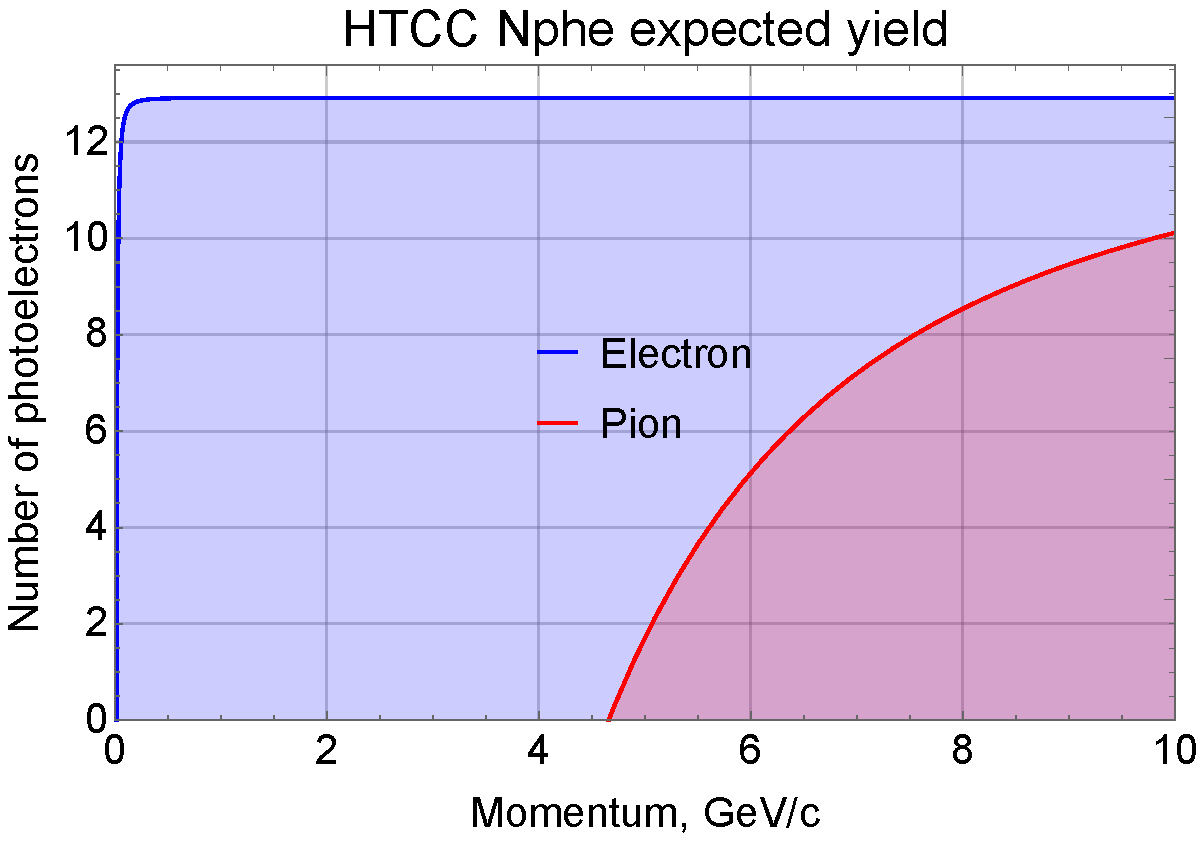
\includegraphics[width=0.45\textwidth]{HTCC.pdf}
\caption{ HTCC $N_{phe}$ expected yield  }
\label{HTCC}
\end{center}
\end{figure} 


Page 17\\
Please provide HTCC response to the simulated pions: $N_{phe}$ as a function od $\theta$ and $\phi$ as in Fig. 2.5.

Page 19, Multivariate analysis\\
MVA requires clean sample for the signal and background. The problem with positron ID appears only for particles with momentum $> 5$ GeV. However, the variables that are used in the analysis (SF, shower profile) have very weak dependence on the particle momentum. It means that we can test the proposed PID method for particles with $P<$ 5 GeV or even apply MVA for low momentum particles. What is wrong with such approach?

Page 26, Eq. 2.16\\
Does pion contamination depend on the reaction kinematics, positron momentum and angles?

Page 29, Fig. 2.21\\
The errors on the bottom plots are calculated incorrectly. It is obvious that the ratio cannot be more than 1.
The correct formula in your case is
\begin{equation}
\begin{split}
        \epsilon&=\frac{N}{N_0}\\
	\sigma(\epsilon)&=\sqrt{\frac{N}{N_0^2}(1-\frac{N}{N_0})}=\sqrt{\frac{\epsilon(1-\epsilon)}{N_0}}
\end{split}
\end{equation}
\noindent
where $N_0$ is the number of the events without cut and $N$ is the number of the events with cut.

Page 30, Fig. 2.22\\
What is the ratio? Nocut/cut or opposite?\\
The same note about the errors of the ratio.

Fig. 2.21, 2.23, 2.26\\
Could you please show the distributions starting from lower momentum (2-3 GeV?)?

Fig. 2.20 and 2.25\\
The MC efficiency (2.20) is close to 100\%. 
Does 2.25 really present the signal efficiency? 
What value of cut was used for the event's selection? 

Page 28-29, lines 543-550\\
I am not sure that the explanation of the low $\pi^-$ contamination (lines 543-550) is the only one possible.
The obvious asymmetry between positrons and electrons is coming from the fact that we have electron beam.
The reaction $ep\to e'p'\pi^+(\pi^-)$ is the source for the $\pi^+$ contamination.
The similar reaction  $ep\to e'p'\pi^-(\pi^+)$ doesn't give the $\pi^-$ contamination because we have $e^-e^-$ final state. 
That is why we don't have $\pi^-$ contamination compatible with $\pi^+$.  The photoproduction
$\gamma p\to'p'\pi^+\pi^-$ doesn't give the signiuficant background because we have to misidentify both particles $\pi^+$  and $\pi^-$. The lepton number conservation has nothing to do with the CLAS12 background I think.

Page 29. Section 2.3\\
Can we apply positron and electron PID for all momenta? What will be the result?

Page 34. Section 2.4.2\\
The data-driven correction are based on the $e',~\pi^+$ and $\pi^-$ momenta measured in the FD. Did you apply corrections to the momenta of these particles? Missing mass fit may help to understand the accuracy of the FD momenta measurements.

Page 39, Fig. 2.38\\
What are the units of the x-axis in the top plots?
Do you have the same plots for positrons?

Page 40, Fig. 2.39 and Fig. 2.40\\
It seams to me that the complicated cuts, based on the mean shower width,  just remove 1 or two counters on the border of the detector in U, V and W strips.

Page 44, Fig 2.43\
Why are the efficiency corrections so irregular? Is it statistics or something else?

Page 48, Eq. 3.5\\
Misprint in the equation: $p_{beam}+p_{target}=....$.

Page 49, Line 815\\
$P_X$ is the x-projection of the $p_{e'}$ probably. In fact it is Z-projection as written in line 828.

Page 50, line 844\\
Usually we use low case letter for $\psi$; $J/\psi$.

Page 52, Line 852\\
Use $\phi$ for $\phi$-meson.

Page 52, Fig. 3.6\\
Is there a possibility to compare cross sections? 

Line 948\\
Misprint: event.

Page 74 Line 1181\\
There is a discrepancy between 3.31b figure capture and text. Probably the corect reference is 3.31d.
The color scheme is not defined.

Page 75, Line 1181\\
Where is it coming from the range $0.5\pm0.1$  in neural network  systematic error study? 
How do you choose the value 0.1?

Page 75, Line 1207\\
Wrong reference to the Fig. 3.31.d. It is 3.31f

Page 76, Lines 1212 and 1214\\
How do you choose the values 0.04 and 0.3 $GeV^2$ for this study?
I would like to note that the FB-asymmetry was changed by $1~\sigma$. 
It is a big step. What will be the result if we will use 0.06 and 0.5 $GeV^2$ cuts?

Fig. 4.1-4.12\\
Can we compare these measurements with the theoretical model predictions?\\
How do you calculate the average values for $<t>,~<M>,~ <E_\gamma>$?
It becomes important when you are trying to compare your data with the theory predictions.
If your average  is just weighted with the cross section (and/or acceptance) value it may give you incorrect result.
This is especially important when the cross section changes significantly inside the kinematic bin. I believe it is your case. 

Let me give you an example. You measure the cross section in the bin $(x_1,x_2)$
$$\bar \sigma=\int_{x_1}^{x_2}\frac{d\sigma}{dx}dx$$
and want to publish diferential cross section 
$$\frac{d\sigma}{dx}=\frac{\bar \sigma}{\Delta x}$$
where $\Delta x=x_2-x_1$.

 The question is: what is correct
value of $\tilde x$ where you want to present your data $\frac{d\sigma}{dx}(\tilde x)$? Very often people 
take the average value weighted with the cross section
$$\bar x=\frac{\int_{x_1}^{x_2}x\frac{d\sigma}{dx}dx}{ \int_{x_1}^{x_2}\frac{d\sigma}{dx}dx}.$$
However this is not correct. You can take the simple example $\frac{d\sigma}{dx}=x$ and $x_1=0$, $x_2=1$.
You will get $\bar x=\frac{2}{3}$. The obvious correct value is 0.5. 

The correct way to get $\tilde x$ is to solve this equation

$$\frac{d\sigma}{dx}(\tilde x)=\frac{\bar \sigma}{\Delta x}$$
You have to know the functional form of your cross section.
You can take it from the theory or from the common consideration for example.

Page 105. Appendix A\\
The background/signal ratio is completely based on the MC. There is no systematic error study connected with this method.

Line 1410\\
There are no Eqs H.1 and H.2 in the text.















\end{document}  